\begin{example}\label{ex:Spoly}
Observe that $w = 378149256$, whose annotated Rothe diagram appears below, is an example of a CDG permutation with a unique lower outside corner  $(i,j) = (6,6)$ and $4=\rank_w(i,j)+1 \neq \min\{m_1,m_2\}=6$.  We illustrate how the reduction of the $s$-polynomial of $h_b = \begin{vmatrix} z_{2,3} & z_{2,4} \\ z_{3,3} & z_{3,4} \end{vmatrix}$ and $\begin{vmatrix} z_{2,3} & z_{2,5} \\ z_{5,3} & z_{5,5} \end{vmatrix}$ gives rise to that of $\begin{vmatrix} z_{2,3} & z_{2,4} \\ z_{3,3} & z_{3,4} \end{vmatrix}$ and $q_a = \begin{vmatrix} 0 & z_{2,3} & z_{2,5} \\ z_{4,2} & z_{4,3} & z_{4,5} \\ z_{5,2} & z_{5,3} & z_{5,5} \end{vmatrix}$ by the process described in Lemma \ref{lem:GrobnerQs}.  Using that \[
z_{5,5} { \color{burntorange}\begin{vmatrix} z_{2,3} & z_{2,4} \\ z_{3,3} & z_{3,4} \end{vmatrix}}-z_{3,4} \begin{vmatrix} z_{2,3} & z_{2,5} \\ z_{5,3} & z_{5,5} \end{vmatrix} +z_{2,4} \begin{vmatrix} z_{3,3} & z_{3,5} \\ z_{5,3} & z_{5,5} \end{vmatrix} + z_{5,3} {\color{burntorange} \begin{vmatrix} z_{2,4} & z_{2,5} \\ z_{3,4} & z_{3,5} \end{vmatrix}} = 0,
\] we construct the equation \begin{align*}
 {\color{blue}\underline{z_{4,2} z_{5,5} \begin{vmatrix} z_{2,3} & z_{2,4} \\ z_{3,3} & z_{3,4} \end{vmatrix}}}+{\color{blue}\underline{z_{3,4}} }\begin{vmatrix} 0 & \color{blue}\underline{z_{2,3}} & \color{blue}\underline{z_{2,5}} \\ \color{blue}\underline{z_{4,2}} & z_{4,3} & z_{4,5} \\  z_{5,2} & \color{blue}\underline{z_{5,3}} & \color{blue}\underline{z_{5,5}} \end{vmatrix}  &- 
  {\color{blue}\underline{z_{2,4}}} \begin{vmatrix} 0 & \color{blue}\underline{z_{3,3}} & \color{blue}\underline{z_{3,5}} \\ \color{blue}\underline{z_{4,2}} & z_{4,3} & z_{4,5} \\ z_{5,2} & \color{blue}\underline{z_{5,3}} & \color{blue}\underline{z_{5,5}} \end{vmatrix}+ {\color{blue}\underline{z_{4,2} z_{5,3} \begin{vmatrix} z_{2,4} & z_{2,5} \\ z_{3,4} & z_{3,5} \end{vmatrix} }}\\
  &= z_{5,2} \left(z_{4,5}   {\color{burntorange}\begin{vmatrix} z_{2,3} & z_{2,4} \\ z_{3,3} & z_{3,4} \end{vmatrix}} +z_{4,3} { \color{burntorange} \begin{vmatrix} z_{2,4} & z_{2,5} \\ z_{3,4} & z_{3,5} \end{vmatrix}}\right).
\end{align*} In the latter equation, we find an $z_{4,2}$-multiple of the first equation (whose terms appear in blue and also are underlined) and an $z_{5,2}$-multiple of an element easily seen to be in $N_{y,I_w}$.  We record in orange the generators of $N_{y,I_w}$ that give the inclusion of the $z_{5,2}$-multiple summand of $s(q_a,h_b)$ in $N_{y,I_w}$ and see that relation arising from the first equation.  The new relation is obtained from the first by exchanging rows $4$ and $5$.  
\[
\hspace{1cm} 
\hspace{0.5cm} 
  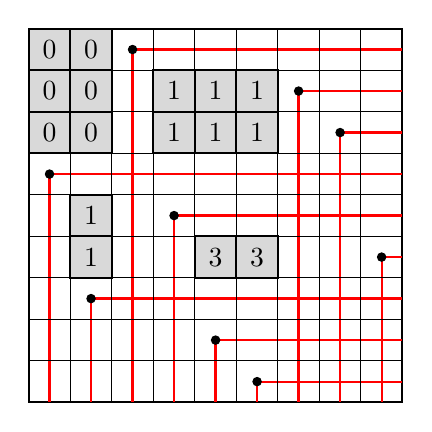
\begin{tikzpicture}[x=1.5em,y=1.5em]
      \draw[color=black, thick](0,1)rectangle(9,10);
     \filldraw[color=black, fill=gray!30, thick](0,9)rectangle(1,10);
      \filldraw[color=black, fill=gray!30, thick](1,9)rectangle(2,10);
      \filldraw[color=black, fill=gray!30, thick](0,7)rectangle(1,8);
      \filldraw[color=black, fill=gray!30, thick](0,8)rectangle(1,9);
      \filldraw[color=black, fill=gray!30, thick](1,8)rectangle(2,9);
      \filldraw[color=black, fill=gray!30, thick](1,7)rectangle(2,8);
      \filldraw[color=black, fill=gray!30, thick](1,4)rectangle(2,5);
     \filldraw[color=black, fill=gray!30, thick](1,5)rectangle(2,6);
      \filldraw[color=black, fill=gray!30, thick](5,4)rectangle(6,5);
       \draw[color=black](1,3)rectangle(2,4);
      \draw[color=black](3,3)rectangle(4,4);  
     \draw[thick,color=red] (9,9.5)--(2.5,9.5)--(2.5,1);
     \draw[thick,color=red] (9,8.5)--(6.5,8.5)--(6.5,1);
     \draw[thick,color=red] (9,5.5)--(3.5,5.5)--(3.5,1);
     \draw[thick,color=red] (9,1.5)--(5.5,1.5)--(5.5,1);
     \draw[thick,color=red] (9,7.5)--(7.5,7.5)--(7.5,1);
     \draw[thick,color=red] (9,2.5)--(4.5,2.5)--(4.5,1);
     \draw[thick,color=red] (9,3.5)--(1.5,3.5)--(1.5,1);
     \draw[thick,color=red] (9,6.5)--(0.5,6.5)--(0.5,1);
     \draw[thick,color=red] (9,4.5)--(8.5,4.5)--(8.5,1);
     \filldraw [black](2.5,9.5)circle(.1);
     \filldraw [black](6.5,8.5)circle(.1);
     \filldraw [black](0.5,6.5)circle(.1);
      \filldraw [black](5.5,1.5)circle(.1);
     \filldraw [black](7.5,7.5)circle(.1);
     \filldraw [black](4.5,2.5)circle(.1);
      \filldraw [black](1.5,3.5)circle(.1);
      \filldraw [black](3.5,5.5)circle(.1);
      \filldraw [black](8.5,4.5)circle(.1);
       \draw[color=black](2,7)rectangle(3,8);
      \filldraw[color=black, fill=gray!30, thick](3,7)rectangle(4,8); 
      \filldraw[color=black, fill=gray!30, thick](4,7)rectangle(5,8);
      \filldraw[color=black, fill=gray!30, thick](5,7)rectangle(6,8); 
      \filldraw[color=black, fill=gray!30, thick](5,8)rectangle(6,9);
      \draw[color=black](5,7)rectangle(6,8); 
     \draw[color=black](2,8)rectangle(3,9);
      \draw[color=black](3,8)rectangle(4,9); 
      \draw[color=black](4,8)rectangle(5,9);
      \draw[color=black](5,8)rectangle(6,9); 
      \draw[color=black](2,6)rectangle(3,7);
      \draw[color=black](0,1)rectangle(1,2);
      \draw[color=black](1,2)rectangle(2,3);
      \draw[color=black](3,4)rectangle(4,5);
      \draw[color=black](1,6)rectangle(2,7);
      \draw[color=black](2,6)rectangle(3,7);
      \filldraw[color=black, fill=gray!30, thick](3,8)rectangle(4,9); 
      \filldraw[color=black, fill=gray!30, thick](4,8)rectangle(5,9);
      \draw[color=black](5,6)rectangle(6,7); 
      \draw[color=black](0,5)rectangle(1,6);
      \draw[color=black](1,5)rectangle(2,6);  
      \draw[color=black](2,5)rectangle(3,6);
      \draw[color=black](3,5)rectangle(4,6); 
      \draw[color=black](4,5)rectangle(5,6);
      \draw[color=black](5,5)rectangle(6,6); 
     \draw[color=black](0,4)rectangle(1,5); 
      \draw[color=black](2,4)rectangle(3,5);
    \filldraw[color=black, fill=gray!30, thick](4,4)rectangle(5,5);
      \draw[color=black](5,4)rectangle(6,5); 
      \draw[color=black](0,3)rectangle(1,4); 
      \draw[color=black](2,3)rectangle(3,4);
      \draw[color=black](4,3)rectangle(5,4);
      \draw[color=black](5,3)rectangle(6,4); 
      \draw[color=black](0,2)rectangle(1,3); 
      \draw[color=black](2,2)rectangle(3,3);
      \draw[color=black](3,2)rectangle(4,3);
      \draw[color=black](4,2)rectangle(5,3);
      \draw[color=black](5,2)rectangle(6,3); 
      \draw[color=black](1,1)rectangle(2,2);  
      \draw[color=black](0,6)rectangle(1,7);  
      \draw[color=black](0,9)rectangle(1,10); 
      \draw[color=black](1,9)rectangle(2,10); 
      \draw[color=black](2,1)rectangle(3,2);
      \draw[color=black](2,9)rectangle(3,10); 
      \draw[color=black](3,1)rectangle(4,2); 
      \draw[color=black](3,9)rectangle(4,10); 
      \draw[color=black](4,1)rectangle(5,2);
      \draw[color=black](4,9)rectangle(5,10); 
      \draw[color=black](5,1)rectangle(6,2); 
      \draw[color=black](5,9)rectangle(6,10); 
      \draw[color=black](6,1)rectangle(7,2); 
      \draw[color=black](6,2)rectangle(7,3); 
      \draw[color=black](6,3)rectangle(7,4); 
      \draw[color=black](6,4)rectangle(7,5); 
      \draw[color=black](6,5)rectangle(7,6); 
      \draw[color=black](6,6)rectangle(7,7); 
      \draw[color=black](6,7)rectangle(7,8); 
      \draw[color=black](6,8)rectangle(7,9);
      \draw[color=black](6,9)rectangle(7,10);  
       \draw[color=black](7,1)rectangle(8,2); 
      \draw[color=black](7,2)rectangle(8,3); 
      \draw[color=black](7,3)rectangle(8,4); 
      \draw[color=black](7,4)rectangle(8,5); 
      \draw[color=black](7,5)rectangle(8,6); 
      \draw[color=black](7,6)rectangle(8,7); 
      \draw[color=black](7,7)rectangle(8,8); 
      \draw[color=black](7,8)rectangle(8,9);
       \draw[color=black](7,9)rectangle(8,10);  
      \draw[color=black](8,1)rectangle(9,2); 
      \draw[color=black](8,2)rectangle(9,3); 
      \draw[color=black](8,3)rectangle(9,4); 
      \draw[color=black](8,4)rectangle(9,5); 
      \draw[color=black](8,5)rectangle(9,6); 
      \draw[color=black](8,6)rectangle(9,7); 
      \draw[color=black](8,7)rectangle(9,8); 
      \draw[color=black](8,8)rectangle(9,9); 
      \draw[color=black](8,9)rectangle(9,10); 
      \draw[color=black](4,5)rectangle(6,7); 
      \node at (0.5,9.5) {$0$};
      \node at (1.5,9.5) {$0$};
      \node at (0.5,7.5) {$0$};
     \node at (1.5,7.5) {$0$};
      \node at (0.5,8.5) {$0$};
      \node at (1.5,8.5) {$0$};
      \node at (1.5,4.5) {$1$};
       \node at (1.5,5.5) {$1$};
       \node at (5.5,4.5) {$3$};
       \node at (4.5,4.5) {$3$};
       \node at (3.5,8.5) {$1$};
       \node at (4.5,8.5) {$1$};
       \node at (3.5,7.5) {$1$};
       \node at (4.5,7.5) {$1$};
       \node at (5.5,7.5) {$1$};
       \node at (5.5,8.5) {$1$};
     \end{tikzpicture}.
       \]
\end{example}
